\icode{E-MV-MU-L2-261011-001}
（多选）
一列沿\(x\)轴正方向传播的简谐横波，\(t = 0\)时，波刚好传播到\(M\)点，波形如图实线所示，\(t =\) \,\qty{0.3}{s}时，波刚好传播到\(N\)点，波形如图虚线所示。则以下说法正确的是\paren[]

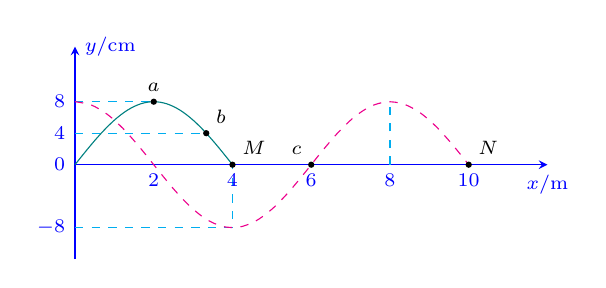
\begin{tikzpicture}[>=stealth,font=\scriptsize]
	\draw[->,blue] (0,0)--(6,0)node[below]{\(x\)/\qty{}{m}};
	\draw[->,blue] (0,-1.2)--(0,1.5)node[right]{\(y\)/\qty{}{cm}};
    \draw[dashed,cyan] (0,.8)--(1,.8)coordinate(a) (0,-.8)--(2,-.8)--(2,0) (0,.4)--({5/3},.4)coordinate(b) (4,0)--(4,.8);   
	\draw[domain=0:5,smooth,dashed,magenta] plot(\x,{.8*cos(.5*pi*\x r)});
	\draw[domain=0:2,smooth,teal] plot(\x,{.8*sin(.5*pi*\x r)});
	\foreach \x/\n in {1/2,2/4,3/6,4/8,5/10}
		\node[blue] at(\x,0)[below]{\(\n\)};
	\foreach \y/\n in{-.8/-8,0/0,.4/4,.8/8}
		\node[blue] at(0,\y)[left]{\(\n\)};
	\fill (a)node[above]{\(a\)} circle(.04) (b)node[above right]{\(b\)} circle(.04) (3,0)node[above left]{\(c\)} circle(.04) (2,0)node[above right]{\(M\)} circle(.04) (5,0)node[above right]{\(N\)} circle(.04);
\end{tikzpicture}
\begin{choices}
	\item 波的周期为\qty{0.6}{s}
	\item 波的波速为\qty{20}{m/s}
	\item \(c\)点在\(0\sim0.3\)\qty{}{s}内通过的路程等于\qty{16}{cm}
	\item \(t =\) \,\qty{0.25}{s}时，\(a\)点与\(M\)点的位移相同
\end{choices}
\begin{answer}
    BC
\end{answer}